% Appendix Stellar Mass Assembly

\chapter{Appendix A. Stellar Mass Assembly: Comparison to other models.}
\label{Appx:StellarMassAssembly}
\lhead{Appendix A. \emph{Stellar Mass Assembly}}

In Figure \ref{fig:SatelliteAccretion_ill} we show the in-situ vs ex-situ growth with the same model as shown in Figure \ref{fig:SatelliteAccretion}, we add to this plot data extracted from the Illustris TNG100 simulation. In Figure \ref{fig:PairFractionIll} we see Illustris has a shallower slow mass slope and a steeper high mass slope such that more stellar mass is mapped into haloes of all sizes. We see the change in both of these slopes reflected in the accretion histories, firstly, for the lower mass galaxies (see $log 10 M_{*,cen} = 10^{11}$)  closer to the SMHM knee we find enhanced accretion due to the larger masses from more minor mergers. Secondly the high mass slope is a direct result of the accretion, to support the same merger assembly with the higher mass galaxies in the satellite haloes above the knee where galaxy growth is dominated by the accretion the galaxy growth with halo size must be enhanced.
 

\begin{figure*}
	\centering
	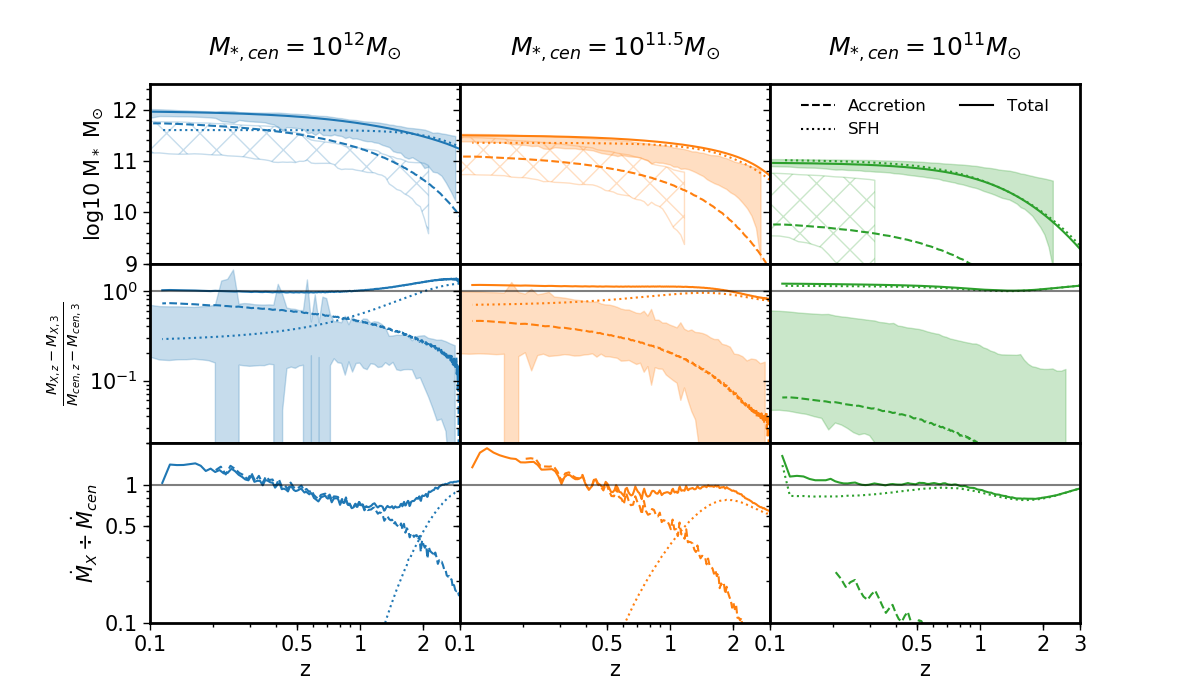
\includegraphics[width = \linewidth]{Appendices/StellarMassAssembly/SatelliteAccretion_G19_ill.png}
    \caption{As in Figure \ref{fig:SatelliteAccretion} three `mass tracks' are shown that have central galaxy masses at redshift $z = 0.1$ of $M_{*,cen}$ = $10^{12}$, $10^{11.5}$, and $10^{11}$ $[M_{\odot}]$ in blue orange and green respectively. The satellite galaxy accretion is shown for evolved satellites with a dashed line and the mass from star formation shown with a dotted line. The top panel shows the total mass of the central (solid line) and the total mass gained from accretion or star formation. The middle panel shows the fraction of the total galaxy mass formed from satellite accretion or star formation since redshift $z=3$. The bottom panel shows the ratio of the mass accretion rate from satellite galaxies the star formation rate and the mass growth rate of the central galaxy predicted by abundance matching. In the top panel the shaded regions are galaxies selected from the Illustris simulation the hashed region is then the satellite accretion from Illustris, in the middle panel the shaded region is the ratio of satellite accretion from Illustris. The grey lines in the second and third panel are at unity, the solid lines showing the sum of the other two factors should therefore be close to or on these lines.}
	\label{fig:SatelliteAccretion_ill}
\end{figure*}

In Figure \ref{fig:SatelliteAccretion_EMERGE} we show the in-situ vs ex-situ growth with the same model as shown in Figure \ref{fig:SatelliteAccretion}, we add to this plot data from the \textsc{emerge} model from \citet{Moster2018Emerge10} shown as black lines. The solid lines show the total galaxy mass followed back selecting populations by mass at redshift $z = 0.1$. The dotted and dashed lines show the amount of galaxy mass formed in-situ and ex-situ respectively. In all cases \textsc{emerge} predicts satellite accretion becomes the dominant mass growth pathway at higher redshifts then \textsc{steel}. In the third column we see that \textsc{emerge} and \textsc{steel} also disagree about the mass growth history of $log 10 M_{*,cen}$ = 11 galaxies, however, both models agree that the dominant mass growth path of galaxies at this mass are in-situ processes.

\begin{figure}
	\centering
	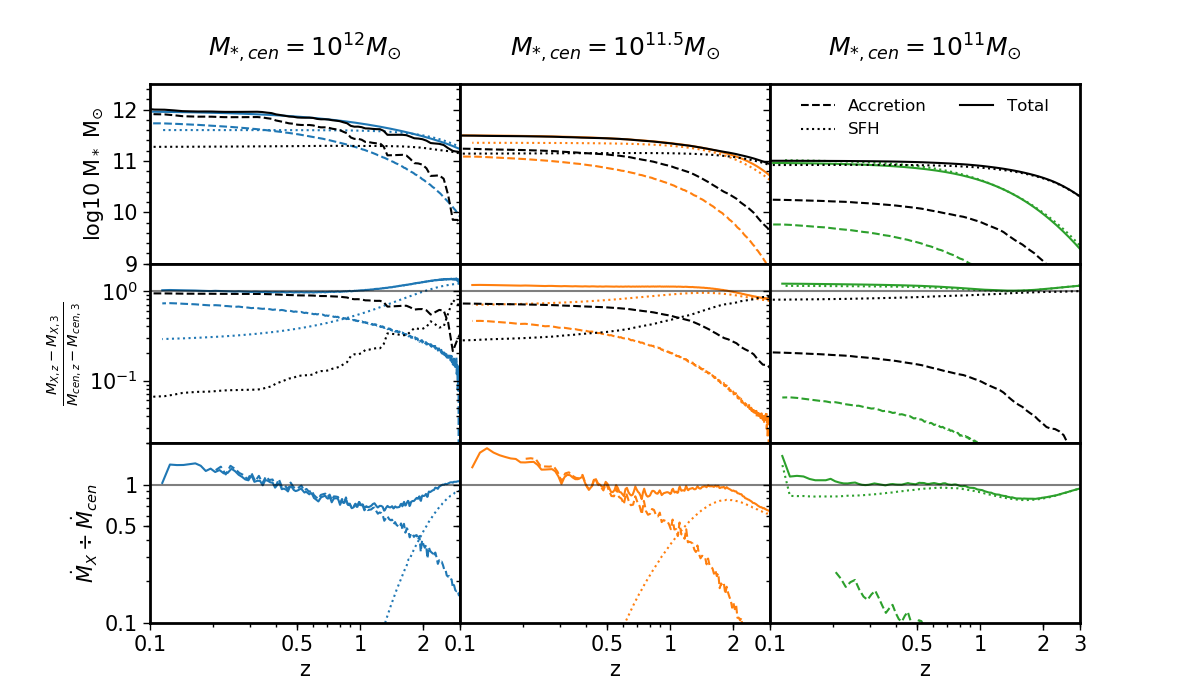
\includegraphics[width = \linewidth]{Appendices/StellarMassAssembly/SatelliteAccretion_EMERGE.png}
    \caption{As in Figure \ref{fig:SatelliteAccretion} three `mass tracks' are shown that have central galaxy masses at redshift $z = 0.1$ of $M_{*,cen}$ = $10^{12}$, $10^{11.5}$, and $10^{11}$ $[M_{\odot}]$ in blue orange and green respectively. The satellite galaxy accretion is shown for evolved satellites with a dashed line and the mass from star formation shown with a dotted line. The top panel shows the total mass of the central (solid line) and the total mass gained from accretion or star formation. The middle panel shows the fraction of the total galaxy mass formed from satellite accretion or star formation since redshift $z=3$. The bottom panel shows the ratio of the mass accretion rate from satellite galaxies the star formation rate and the mass growth rate of the central galaxy predicted by abundance matching. In the top and middle rows we add black lines to show the in-situ and ex-situ growth from \textsc{emerge} \citet{Moster2018Emerge10}. The grey lines in the second and third panel are at unity, the solid lines showing the sum of the other two factors should therefore be close to or on these lines.}
	\label{fig:SatelliteAccretion_EMERGE}
\end{figure}

In Figure \ref{fig:SatelliteAccretion_UniM} we show for the $log 10 M_{*,cen}$ = 11.5, and 11 galaxies the central growth and star formation rate ratio from \citet{Behroozi2019UniverseMachine:010}. The central growth is close to that found from \textsc{steel} and the star formation rate transition for  $log 10 M_{*,cen}$ = 11.5 is an excellent match.

\begin{figure*}
	\centering
	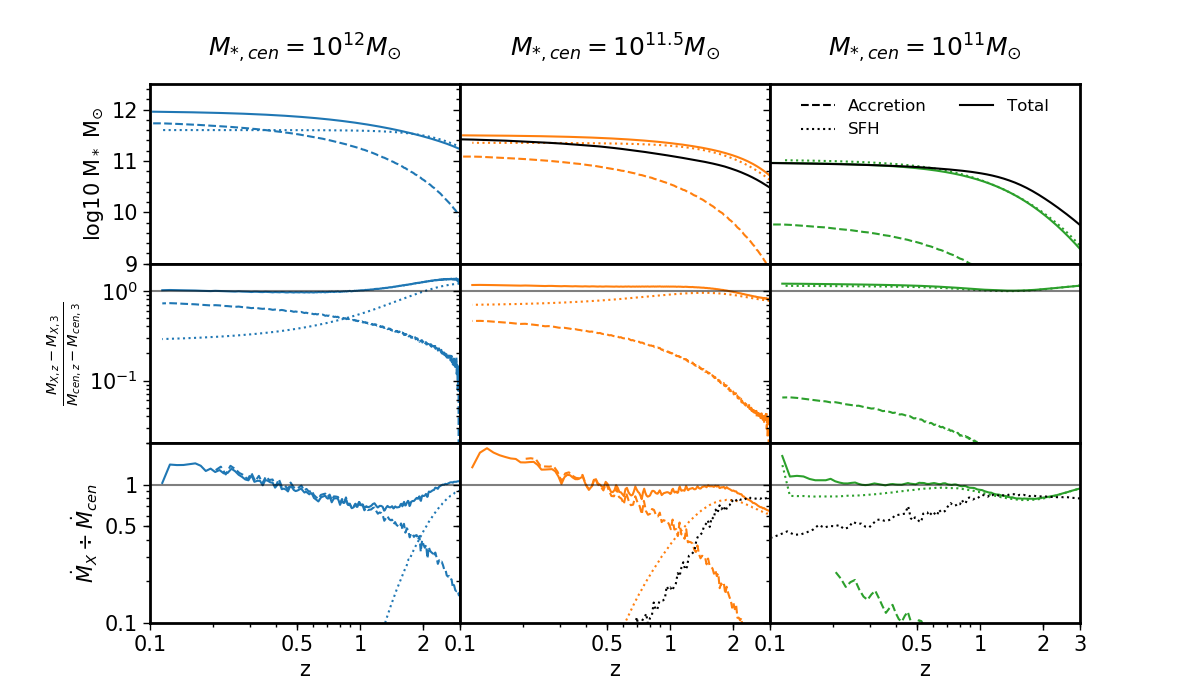
\includegraphics[width = \linewidth]{Appendices/StellarMassAssembly/SatelliteAccretion_UniM.png}
    \caption{As in Figure \ref{fig:SatelliteAccretion} three `mass tracks' are shown that have central galaxy masses at redshift $z = 0.1$ of $M_{*,cen}$ = $10^{12}$, $10^{11.5}$, and $10^{11}$ $[M_{\odot}]$ in blue orange and green respectively. The satellite galaxy accretion is shown for evolved satellites with a dashed line and the mass from star formation shown with a dotted line. The top panel shows the total mass of the central (solid line) and the total mass gained from accretion or star formation. The middle panel shows the fraction of the total galaxy mass formed from satellite accretion or star formation since redshift $z=3$. The bottom panel shows the ratio of the mass accretion rate from satellite galaxies the star formation rate and the mass growth rate of the central galaxy predicted by abundance matching. In the top and bottom rows, for the $log 10 M_{*,cen}$ = 11.5, and 11, we add black lines to show the central galaxy growth and the star formation rate ratio from \citet{Behroozi2019UniverseMachine:010}. The grey lines in the second and third panel are at unity, the solid lines showing the sum of the other two factors should therefore be close to or on these lines.}
	\label{fig:SatelliteAccretion_UniM}
\end{figure*}

In Figure \ref{fig:SatelliteAccretion_Menci} we show a comparison with the Semi-Analytic model described in \citet{Menci2014TriggeringInteractions}. At all masses the stellar growth is substantially different to \textsc{steel} and the other models shown in this appendix. Furthermore the Semi-Analytic model shows little change in the accreted mass ratio over cosmic time, again this is inconsistent with the findings from \textsc{steel} and the other models presented in this section. We attribute most of the differences seen here to the substantial difference in the SMHM relationship between the two models.

\begin{figure*}
	\centering
	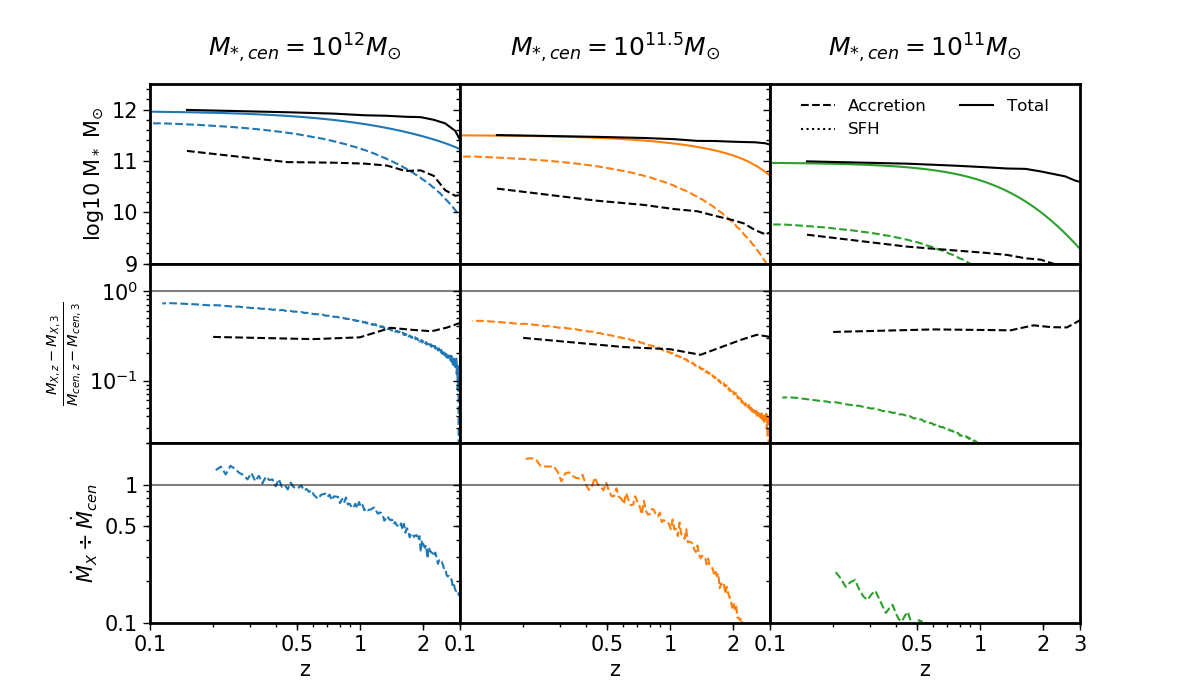
\includegraphics[width = \linewidth]{Appendices/StellarMassAssembly/SatelliteAccretion_Menci.png}
    \caption{As in Figure \ref{fig:SatelliteAccretion} three `mass tracks' are shown that have central galaxy masses at redshift $z = 0.1$ of $M_{*,cen}$ = $10^{12}$, $10^{11.5}$, and $10^{11}$ $[M_{\odot}]$ in blue orange and green respectively. The satellite galaxy accretion is shown for evolved satellites with a dashed line and the mass from star formation shown with a dotted line. The top panel shows the total mass of the central (solid line) and the total mass gained from accretion or star formation. The middle panel shows the fraction of the total galaxy mass formed from satellite accretion or star formation since redshift $z=3$. The bottom panel shows the ratio of the mass accretion rate from satellite galaxies the star formation rate and the mass growth rate of the central galaxy predicted by abundance matching. In the top and middle rows we add black lines to show the ex-situ growth and central growth from the Semi-Analytic model described in \citet{Menci2014TriggeringInteractions}. The grey lines in the second and third panel are at unity, the solid lines showing the sum of the other two factors should therefore be close to or on these lines.}
	\label{fig:SatelliteAccretion_Menci}
\end{figure*}